% questions.tex —— 2016 年·全国Ⅲ卷·文科 · 题目内容片段（无答案）
% 由 tools/generate_projects.py 依来源总账自 2016/2016_数学真题_全国3文_试题.md 生成，勿手改（改源 MD 后重跑）


\gkpart{数学}

\begin{gktip}
\textbf{来源说明}：本题面依据固定源 PDF 两页 A3 页面逐题核对，原卷印刷页码 1009–1010。固定源不附答案；本文件仅为题面规范源。未决答案不影响题面忠实呈现，详见答案与问题总账。
\end{gktip}

\gkpart{一、选择题}

\begin{question}
\gkti{1}设集合 \(A=\{0,2,4,6,8,10\}\)，\(B=\{4,8\}\)，则 \(\complement_A B=\)（　）

（A）\(\{4,8\}\)　（B）\(\{0,2,6\}\)　（C）\(\{0,2,6,10\}\)　（D）\(\{0,2,4,6,8,10\}\)

\end{question}
\begin{question}
\gkti{2}若 \(z=4+3i\)，则 \(\dfrac{\bar z}{|z|}=\)（　）

（A）\(1\)　（B）\(-1\)　（C）\(\dfrac45+\dfrac35i\)　（D）\(\dfrac45-\dfrac35i\)

\end{question}
\begin{question}
\gkti{3}已知向量 \(\overrightarrow{BA}=\left(\dfrac12,\dfrac{\sqrt3}{2}\right)\)，\(\overrightarrow{BC}=\left(\dfrac{\sqrt3}{2},\dfrac12\right)\)，则 \(\angle ABC=\)（　）

（A）\(30^\circ\)　（B）\(45^\circ\)　（C）\(60^\circ\)　（D）\(120^\circ\)

\Needspace{0.4\textheight}
\end{question}
\begin{question}
\gkti{4}某旅游城市为向游客介绍本地的气温情况，绘制了一年中月平均最高气温和平均最低气温的雷达图。图中 \(A\) 点表示十月的平均最高气温约为 \(15^\circ\mathrm C\)，\(B\) 点表示四月的平均最低气温约为 \(5^\circ\mathrm C\)。下面叙述不正确的是（　）
\nopagebreak[4]
\begin{center}\begin{tikzpicture}[scale=0.75,line cap=round,line join=round,font=\small]
% 折线坐标按固定原 PDF 的矢量路径等比例重绘，不作为逐月精确数据表。
\foreach \r/\lab in {0.6/5,1.2/10,1.8/15,2.4/20}{\draw[gray!65] (0,0) circle (\r);\node[anchor=west,inner sep=1pt] at (0.05,\r) {\scriptsize \lab$^\circ$C};}
\draw[gray!65] (0,0) circle (3);
\foreach \i/\m in {0/一月,1/二月,2/三月,3/四月,4/五月,5/六月,6/七月,7/八月,8/九月,9/十月,10/十一月,11/十二月}{\draw[gray!60] (0,0)--({90-30*\i}:3);\node at ({90-30*\i}:3.35) {\m};}
\draw[thick,fill=black,fill opacity=0.10] (1.800,0)--(1.039,0.600)--(0.450,0.780)--(0,0.780)--(-0.420,0.727)--(-1.039,0.600)--(-1.800,0)--(-1.923,-1.110)--(-1.380,-2.390)--(0,-2.640)--(1.200,-2.078)--(1.923,-1.110)--cycle;
\draw[densely dashed,thick,fill=black,fill opacity=0.10] (0.600,0)--(0.208,0.120)--(0.090,0.156)--(0,0.300)--(-0.210,0.364)--(-0.520,0.300)--(-1.200,0)--(-1.195,-0.690)--(-0.780,-1.351)--(0,-1.500)--(0.600,-1.039)--(0.779,-0.450)--cycle;
\foreach \x/\y in {1.800/0,1.039/0.600,0.450/0.780,0/0.780,-0.420/0.727,-1.039/0.600,-1.800/0,-1.923/-1.110,-1.380/-2.390,0/-2.640,1.200/-2.078,1.923/-1.110,0.600/0,0.208/0.120,0.090/0.156,0/0.300,-0.210/0.364,-0.520/0.300,-1.200/0,-1.195/-0.690,-0.780/-1.351,0/-1.500,0.600/-1.039,0.779/-0.450}{\fill (\x,\y) circle (1pt);}
\foreach \i in {1,...,24}{\draw[thin] (0,{0.12*\i})--(-0.06,{0.12*\i});}
\fill (-1.800,0) circle (1.2pt) node[above left] {$A$};
\fill (0.600,0) circle (1.2pt) node[above right] {$B$};
\draw[thick] (-1.8,-3.95)--(-1.4,-3.95) node[right]{平均最高气温};
\draw[densely dashed] (-1.8,-4.60)--(-1.4,-4.60) node[right]{平均最低气温};
\end{tikzpicture}
\end{center}
\nopagebreak[4]
（A）各月的平均最低气温都在 \(0^\circ\mathrm C\) 以上

（B）七月的平均温差比一月的平均温差大

（C）三月和十一月的平均最高气温基本相同

（D）平均气温高于 \(20^\circ\mathrm C\) 的月份有 5 个

\end{question}
\begin{question}
\gkti{5}小敏打开计算机时，忘记了开机密码的前两位，只记得第一位是 \(M,I,N\) 中的一个字母，第二位是 \(1,2,3,4,5\) 中的一个数字，则小敏输入一次密码能够成功开机的概率是（　）

（A）\(\dfrac8{15}\)　（B）\(\dfrac18\)　（C）\(\dfrac1{15}\)　（D）\(\dfrac1{30}\)

\end{question}
\begin{question}
\gkti{6}若 \(\tan\theta=-\dfrac13\)，则 \(\cos2\theta=\)（　）

（A）\(-\dfrac45\)　（B）\(-\dfrac15\)　（C）\(\dfrac15\)　（D）\(\dfrac45\)

\end{question}
\begin{question}
\gkti{7}已知 \(a=2^{\frac43}, b=3^{\frac23}, c=25^{\frac13}\)，则（　）

（A）\(b<a<c\)　（B）\(a<b<c\)　（C）\(b<c<a\)　（D）\(c<a<b\)

\Needspace{0.4\textheight}
\end{question}
\begin{question}
\gkti{8}执行如图所示的程序框图，如果输入的 \(a=4,b=6\)，那么输出的 \(n=\)（　）
\nopagebreak[4]
\begin{center}\begin{tikzpicture}[node distance=4mm and 13mm, every node/.style={font=\small},
  term/.style={draw,rounded corners,minimum width=1.5cm,minimum height=6mm},
  box/.style={draw,minimum width=2.8cm,minimum height=6mm},
  io/.style={draw,trapezium,trapezium left angle=70,trapezium right angle=110,minimum width=2.8cm,minimum height=6mm},decision/.style={draw,diamond,aspect=2.1,inner sep=1pt}]
\node[term] (start) {开始};
\node[io,below=of start] (input) {输入 $a,b$};
\node[box,below=of input] (init) {$n=0,\ s=0$};
\node[box,below=of init] (a1) {$a=b-a$};
\node[box,below=of a1] (b1) {$b=b-a$};
\node[box,below=of b1] (a2) {$a=b+a$};
\node[box,below=of a2] (sum) {$s=s+a,\ n=n+1$};
\node[decision,below=of sum] (test) {$s>16$};
\node[io,below=of test] (out) {输出 $n$};
\node[term,below=of out] (end) {结束};
\draw[->] (start)--(input);
\draw[->] (input)--(init);
\draw[->] (init)--(a1);
\draw[->] (a1)--(b1);
\draw[->] (b1)--(a2);
\draw[->] (a2)--(sum);
\draw[->] (sum)--(test);
\draw[->] (test.south)--node[right]{是}(out.north);
\draw[->] (out)--(end);
\draw[->] (test.west)--node[above]{否} ++(-1.3,0) |- (a1.west);
\end{tikzpicture}
\end{center}
\nopagebreak[4]
（A）3　（B）4　（C）5　（D）6

\end{question}
\begin{question}
\gkti{9}在 \(\triangle ABC\) 中，\(B=\dfrac\pi4\)，\(BC\) 边上的高等于 \(\dfrac13BC\)，则 \(\sin A=\)（　）

（A）\(\dfrac3{10}\)　（B）\(\dfrac{\sqrt{10}}{10}\)　（C）\(\dfrac{\sqrt5}{5}\)　（D）\(\dfrac{3\sqrt{10}}{10}\)

\Needspace{0.4\textheight}
\end{question}
\begin{question}
\gkti{10}如图，网格纸上小正方形的边长为 1，粗实线画出的是某多面体的三视图，则该多面体的表面积为（　）
\nopagebreak[4]
\begin{center}
\begin{tikzpicture}[scale=0.32,line width=1.1pt,line cap=round,line join=round]
% 固定原 PDF 矢量网格为 13×13；侧投影高度 6 格。
\draw[step=1,gray!45,very thin] (0,0) grid (13,13);
\draw (1,6)--(4,12)--(7,12)--(4,6)--cycle;
\draw (9,6) rectangle (12,12);
\draw (1,1) rectangle (7,4);
\draw (4,1)--(4,4);
\end{tikzpicture}
\end{center}
\nopagebreak[4]
（A）\(18+36\sqrt5\)　（B）\(54+18\sqrt5\)　（C）\(90\)　（D）\(81\)

\end{question}
\begin{question}
\gkti{11}在封闭的直三棱柱 \(ABC-A_1B_1C_1\) 内有一个体积为 \(V\) 的球，若 \(AB\perp BC\)，\(AB=6\)，\(BC=8\)，\(AA_1=3\)，则 \(V\) 的最大值是（　）

（A）\(4\pi\)　（B）\(\dfrac{9\pi}{2}\)　（C）\(6\pi\)　（D）\(\dfrac{32\pi}{3}\)

\end{question}
\begin{question}
\gkti{12}已知 \(O\) 为坐标原点，\(F\) 是椭圆 \(C:\dfrac{x^2}{a^2}+\dfrac{y^2}{b^2}=1\ (a>b>0)\) 的左焦点，\(A,B\) 分别为 \(C\) 的左、右顶点，\(P\) 为 \(C\) 上一点，且 \(PF\perp x\) 轴。过点 \(A\) 的直线 \(l\) 与线段 \(PF\) 交于点 \(M\)，与 \(y\) 轴交于点 \(E\)。若直线 \(BM\) 经过 \(OE\) 的中点，则 \(C\) 的离心率为（　）

（A）\(\dfrac13\)　（B）\(\dfrac12\)　（C）\(\dfrac23\)　（D）\(\dfrac34\)

\end{question}
\gkpart{二、填空题}

\begin{question}
\gkti{13}若 \(x,y\) 满足约束条件
\nopagebreak[4]
\[
\begin{cases}
2x-y+1\geq0,\\
x-2y-1\leq0,\\
x\leq1,
\end{cases}
\]
则 \(z=2x+3y-5\) 的最小值为\gkblank{}。

\end{question}
\begin{question}
\gkti{14}函数 \(y=\sin x-\sqrt3\cos x\) 的图象可由函数 \(y=2\sin x\) 的图象至少向右平移\gkblank{}个单位长度得到。

\end{question}
\begin{question}
\gkti{15}已知直线 \(l:x-\sqrt3y+6=0\) 与圆 \(x^2+y^2=12\) 交于 \(A,B\) 两点，过 \(A,B\) 分别作 \(l\) 的垂线与 \(x\) 轴交于 \(C,D\) 两点，则 \(|CD|=\)\gkblank{}。

\end{question}
\begin{question}
\gkti{16}已知 \(f(x)\) 为偶函数，当 \(x\leq0\) 时，\(f(x)=e^{-x-1}-x\)，则曲线 \(y=f(x)\) 在点 \((1,2)\) 处的切线方程是\gkblank{}。

\end{question}
\gkpart{三、解答题}

\begin{question}
\gkti{17}已知各项都为正数的数列 \(\{a_n\}\) 满足 \(a_1=1\)，\(a_n^2-(2a_{n+1}-1)a_n-2a_{n+1}=0\)。

（1） 求 \(a_2,a_3\)；

（2） 求 \(\{a_n\}\) 的通项公式。

\Needspace{0.4\textheight}
\end{question}
\begin{question}
\gkti{18}下图是我国 2008 年至 2014 年生活垃圾无害化处理量（单位：亿吨）的折线图。
\nopagebreak[4]
\begin{center}\begin{tikzpicture}[x=0.75cm,y=3.0cm,line cap=round,line join=round,font=\small]
% 图示点位取固定原 PDF 折线路径；计算采用题给汇总量。
\draw[->] (0,0.8)--(7.9,0.8) node[right] {$t$};
\draw[->] (0,0.8)--(0,1.96) node[above] {$y$（亿吨）};
\foreach \y in {1.0,1.2,1.4,1.6,1.8}{\draw[densely dashed,gray] (0,\y)--(7.8,\y);\node[left] at (0,\y) {\scriptsize \y};}
\node[left] at (0,0.8) {\scriptsize 0.8};
\foreach \x in {1,...,7}{\draw (\x,0.8)--(\x,0.82);\node[below] at (\x,0.8) {\x};}
\draw plot coordinates {(1,1.04)(2,1.14)(3,1.24)(4,1.32)(5,1.46)(6,1.54)(7,1.62)};
\foreach \x/\y in {1/1.04,2/1.14,3/1.24,4/1.32,5/1.46,6/1.54,7/1.62}{\node[fill,rectangle,inner sep=0.8pt] at (\x,\y) {};}
\end{tikzpicture}
\end{center}
\nopagebreak[4]
注：年份代码 \(1-7\) 分别对应年份 2008–2014。

（1） 由折线图看出，可用线性回归模型拟合 \(y\) 与 \(t\) 的关系，请用相关系数加以说明；

（2） 建立 \(y\) 关于 \(t\) 的回归方程（系数精确到 0.01），预测 2016 年我国生活垃圾无害化处理量。

参考数据：\(\displaystyle\sum_{i=1}^7 y_i=9.32\)，\(\displaystyle\sum_{i=1}^7t_i y_i=40.17\)，\(\displaystyle\sqrt{\sum_{i=1}^7(y_i-\bar y)^2}=0.55\)，\(\sqrt7\approx2.646\)。

参考公式：相关系数 \(\displaystyle r=\frac{\sum_{i=1}^n(t_i-\bar t)(y_i-\bar y)}{\sqrt{\sum_{i=1}^n(t_i-\bar t)^2\sum_{i=1}^n(y_i-\bar y)^2}}\)。回归方程 \(\hat y=\hat a+\hat bt\) 中，\(\displaystyle\hat b=\frac{\sum_{i=1}^n(t_i-\bar t)(y_i-\bar y)}{\sum_{i=1}^n(t_i-\bar t)^2}\)，\(\hat a=\bar y-\hat b\bar t\)。

\Needspace{0.4\textheight}
\end{question}
\begin{question}
\gkti{19}如图，在四棱锥 \(P-ABCD\) 中，\(PA\perp\) 平面 \(ABCD\)，\(AD\parallel BC\)，\(AB=AD=AC=3\)，\(PA=BC=4\)，\(M\) 为线段 \(AD\) 上一点，\(AM=2MD\)，\(N\) 为 \(PC\) 的中点。
\nopagebreak[4]
\begin{center}\begin{tikzpicture}[scale=0.9,line cap=round,line join=round,font=\small]
% 原卷投影等比例重绘；M、N 按题给分点关系定位。
\coordinate (B) at (0,0);
\coordinate (A) at (1.666,0.437);
\coordinate (C) at (2.604,-0.243);
\coordinate (D) at (3.672,0.243);
\coordinate (P) at (1.666,3.154);
\coordinate (M) at ($(A)!2/3!(D)$);
\coordinate (N) at ($(P)!0.5!(C)$);
\draw (P)--(B)--(C)--(D)--(P) (P)--(C) (B)--(N);
\draw[dashed] (P)--(A) (A)--(B) (A)--(C) (A)--(D) (B)--(M) (N)--(M) (M)--(C);
\foreach \pt/\pos in {P/above,A/left,B/left,C/below,D/right,M/right,N/right}{\node[\pos] at (\pt) {$\pt$};}
\end{tikzpicture}
\end{center}
\nopagebreak[4]
（1） 证明：\(MN\parallel\) 平面 \(PAB\)；

（2） 求四面体 \(N-BCM\) 的体积。

\end{question}
\begin{question}
\gkti{20}已知抛物线 \(C:y^2=2x\) 的焦点为 \(F\)，平行于 \(x\) 轴的两条直线 \(l_1,l_2\) 分别交 \(C\) 于 \(A,B\) 两点，交 \(C\) 的准线于 \(P,Q\) 两点。

（1） 若 \(F\) 在线段 \(AB\) 上，\(R\) 是 \(PQ\) 的中点，证明 \(AR\parallel FQ\)；

（2） 若 \(\triangle PQF\) 的面积是 \(\triangle ABF\) 的面积的两倍，求 \(AB\) 中点的轨迹方程。

\end{question}
\begin{question}
\gkti{21}设函数 \(f(x)=\ln x-x+1\)。

（1） 讨论 \(f(x)\) 的单调性；

（2） 证明当 \(x\in(1,+\infty)\) 时，\(1<\dfrac{x-1}{\ln x}<x\)；

（3） 设 \(c>1\)，证明当 \(x\in(0,1)\) 时，\(1+(c-1)x>c^x\)。

\Needspace{0.4\textheight}
\end{question}
\begin{question}
\gkti{22}如图，\(\odot O\) 中弧 \(AB\) 的中点为 \(P\)，弦 \(PC,PD\) 分别交 \(AB\) 于 \(E,F\) 两点。
\nopagebreak[4]
\begin{center}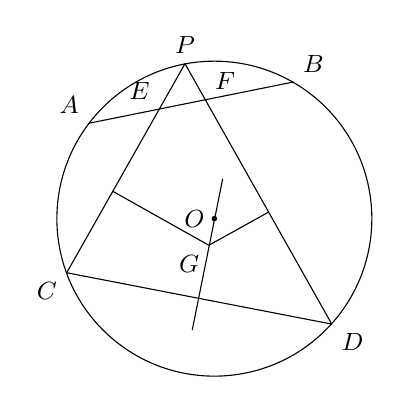
\begin{tikzpicture}[line cap=round,line join=round,font=\small]
% 轮廓及辅助线取固定原 PDF 矢量坐标；交点按直线交点定位。
\draw (0,0) circle (2);
\coordinate (O) at (0,0);
\coordinate (A) at (-1.596,1.211);
\coordinate (B) at (1.002,1.735);
\coordinate (P) at (-0.373,1.968);
\coordinate (C) at (-1.875,-0.687);
\coordinate (D) at (1.491,-1.339);
\coordinate (E) at (intersection of A--B and P--C);
\coordinate (F) at (intersection of A--B and P--D);
\coordinate (G) at (-0.070,-0.338);
\draw (A)--(B) (P)--(C) (P)--(D) (C)--(D);
\draw (0.105,0.501)--(-0.280,-1.409);
\draw (G)--(-1.293,0.349) (G)--(0.687,0.082);
\foreach \pt/\pos in {A/above left,B/above right,C/below left,D/below right,P/above,E/above left,F/above right,O/left,G/below left}{\node[\pos] at (\pt) {$\pt$};}
\fill (O) circle (1pt);
\end{tikzpicture}
\end{center}
\nopagebreak[4]
（1） 若 \(\angle PFB=2\angle PCD\)，求 \(\angle PCD\) 的大小；

（2） 若 \(EC\) 的垂直平分线与 \(FD\) 的垂直平分线交于点 \(G\)，证明 \(OG\perp CD\)。

\end{question}
\begin{question}
\gkti{23}在直角坐标系 \(xOy\) 中，曲线 \(C_1\) 的参数方程为
\nopagebreak[4]
\[
\begin{cases}
x=\sqrt3\cos\alpha,\\
y=\sin\alpha,
\end{cases}
\qquad(\alpha\text{ 为参数}),
\]
以坐标原点为极点、\(x\) 轴的正半轴为极轴建立极坐标系，曲线 \(C_2\) 的极坐标方程为 \(\rho\sin\left(\theta+\dfrac\pi4\right)=2\sqrt2\)。

（1） 写出 \(C_1\) 的普通方程和 \(C_2\) 的直角坐标方程；

（2） 设点 \(P\) 在 \(C_1\) 上，点 \(Q\) 在 \(C_2\) 上，求 \(|PQ|\) 的最小值及此时 \(P\) 的直角坐标。

\end{question}
\begin{question}
\gkti{24}已知函数 \(f(x)=|2x-a|+a\)。

（1） 当 \(a=2\) 时，求不等式 \(f(x)\leq6\) 的解集；

（2） 设函数 \(g(x)=|2x-1|\)，当 \(x\in\mathbb R\) 时，\(f(x)+g(x)\geq3\)，求 \(a\) 的取值范围。

\end{question}